\documentclass[12pt]{article}
\usepackage[utf8]{inputenc}
\usepackage[utf8]{inputenc}
\usepackage{amsmath}
\usepackage{amsthm}
\usepackage{amssymb}
\usepackage{array}
\usepackage{geometry}
\usepackage{amsfonts}
\usepackage{mathrsfs}
\usepackage{bm}
\usepackage{hyperref}
\usepackage{float}
\usepackage[dvipsnames]{xcolor}
\usepackage[inline]{enumitem}
\usepackage{mathtools}
\usepackage{changepage}
\usepackage{graphicx}
\usepackage{systeme}
\usepackage{caption}
\usepackage{subcaption}
\usepackage{lipsum}
\usepackage{tikz}
\usetikzlibrary{matrix, patterns, decorations.pathreplacing, calligraphy}
\usepackage{tikz-cd}
\usepackage[nameinlink]{cleveref}
\geometry{
headheight=15pt,
left=60pt,
right=60pt
}
\setlength{\emergencystretch}{20pt}
\usepackage{fancyhdr}
\pagestyle{fancy}
\fancyhf{}
\lhead{}
\chead{Section 6.7 Exercises}
\rhead{\thepage}
\hypersetup{
    colorlinks=true,
    linkcolor=blue,
    urlcolor=blue
}

\theoremstyle{definition}
\newtheorem*{remark}{Remark}

\newtheoremstyle{exercise}
    {}
    {}
    {}
    {}
    {\bfseries}
    {.}
    { }
    {\thmname{#1}\thmnumber{#2}\thmnote{ (#3)}}
\theoremstyle{exercise}
\newtheorem{exercise}{Exercise 6.7.}

\newtheoremstyle{solution}
    {}
    {}
    {}
    {}
    {\itshape\color{magenta}}
    {.}
    { }
    {\thmname{#1}\thmnote{ #3}}
\theoremstyle{solution}
\newtheorem*{solution}{Solution}

\Crefformat{exercise}{#2Exercise 6.7.#1#3}

\newcommand{\interior}[1]{%
  {\kern0pt#1}^{\mathrm{o}}%
}
\newcommand{\ts}{\textsuperscript}
\newcommand{\setcomp}[1]{#1^{\mathsf{c}}}
\newcommand{\poly}{\mathcal{P}}
\newcommand{\quand}{\quad \text{and} \quad}
\newcommand{\quimplies}{\quad \implies \quad}
\newcommand{\quiff}{\quad \iff \quad}
\newcommand{\upd}{\,\text{d}}
\newcommand{\N}{\mathbf{N}}
\newcommand{\Z}{\mathbf{Z}}
\newcommand{\Q}{\mathbf{Q}}
\newcommand{\I}{\mathbf{I}}
\newcommand{\R}{\mathbf{R}}
\newcommand{\C}{\mathbf{C}}

\DeclarePairedDelimiter\abs{\lvert}{\rvert}
% Swap the definition of \abs* and \norm*, so that \abs
% and \norm resizes the size of the brackets, and the 
% starred version does not.
\makeatletter
\let\oldabs\abs
\def\abs{\@ifstar{\oldabs}{\oldabs*}}
%
\let\oldnorm\norm
\def\norm{\@ifstar{\oldnorm}{\oldnorm*}}
\makeatother

\DeclarePairedDelimiter\paren{(}{)}
\makeatletter
\let\oldparen\paren
\def\paren{\@ifstar{\oldparen}{\oldparen*}}
\makeatother

\DeclarePairedDelimiter\bkt{[}{]}
\makeatletter
\let\oldbkt\bkt
\def\bkt{\@ifstar{\oldbkt}{\oldbkt*}}
\makeatother

\DeclarePairedDelimiter\set{\{}{\}}
\makeatletter
\let\oldset\set
\def\set{\@ifstar{\oldset}{\oldset*}}
\makeatother

\setlist[enumerate,1]{label={(\alph*)}}

\begin{document}

\section{Section 6.7 Exercises}

Exercises with solutions from Section 6.7 of \hyperlink{ua}{[UA]}.

\begin{exercise}
\label{ex:1}
    Assuming WAT, show that if \( f \) is continuous on \( [a, b] \), then there exists a sequence \( (p_n) \) of polynomials such that \( p_n \to f \) uniformly on \( [a, b] \).
\end{exercise}

\begin{solution}
    The Weierstrass Approximation Theorem implies that for each \( n \in \N \) there exists a polynomial \( p_n \) such that
    \[
        \abs{f(x) - p_n(x)} < \frac{1}{n}
    \]
    for all \( x \in [a, b] \). It follows that \( p_n \to f \) uniformly on \( [a, b] \).
\end{solution}

\begin{exercise}
\label{ex:2}
    Prove Theorem 6.7.3.
\end{exercise}

\begin{solution}
    Since \( f \) is a continuous function defined on the compact set \( [a, b] \), Theorem 4.4.7 implies that \( f \) is uniformly continuous on \( [a, b] \) and hence there exists a \( \delta > 0 \) such that
    \[
        x, y \in [a, b] \text{ and } \abs{x - y} < \delta \quimplies \abs{f(x) - f(y)} < \frac{\epsilon}{2}.
    \]
    Let \( n \in \N \) be such that \( \tfrac{1}{n} < \delta \) and for each \( 0 \leq j \leq n \) let \( x_j = a + j \tfrac{b - a}{n} \). Let \( \phi : [a, b] \to \R \) be the polygonal function which is linear on each subinterval \( [x_j, x_{j+1}] \) and passes through the points \( (x_j, f(x_j)) \) and \( (x_{j+1}, f(x_{j+1})) \). For \( x \in [a, b] \), we have \( x \in [x_j, x_{j+1}] \) for some \( 0 \leq j \leq n - 1 \). It follows that
    \[
        \abs{f(x) - \phi(x)} \leq \abs{f(x) - \phi(x_j)} + \abs{\phi(x_j) - \phi(x)} \leq \abs{f(x) - \phi(x_j)} + \abs{\phi(x_j) - \phi(x_{j+1})};
    \]
    for the last inequality we are using that \( \phi \) is a line segment on the interval \( [x_j, x_{j+1}] \) and thus \( \abs{\phi(x) - \phi(y)} \leq \abs{\phi(x_j) - \phi(x_{j+1})} \) for any \( x, y \in [x_j, x_{j+1}] \). By definition we have \( \phi(x_j) = f(x_j) \) for any \( j \) and so
    \[
        \abs{f(x) - \phi(x)} \leq \abs{f(x) - f(x_j)} + \abs{f(x_j) - f(x_{j+1})} < \frac{\epsilon}{2} + \frac{\epsilon}{2} = \epsilon.
    \]
\end{solution}

\begin{exercise}
\label{ex:3}
    \begin{enumerate}
        \item Find the second degree polynomial \( p(x) = q_0 + q_1 x + q_2 x^2 \) that interpolates the three points \( (-1, 1), (0, 0), \) and \( (1, 1) \) on the graph of \( g(x) = \abs{x} \). Sketch \( g(x) \) and \( p(x) \) over \( [-1, 1] \) on the same set of axes.

        \item Find the fourth degree polynomial that interpolates \( g(x) = \abs{x} \) at the points \( x = -1, -1/2, 0, 1/2, \) and 1. Add a sketch of this polynomial to the graph from (a).
    \end{enumerate}
\end{exercise}

\begin{solution}
    \begin{figure}[H]
        \centering
        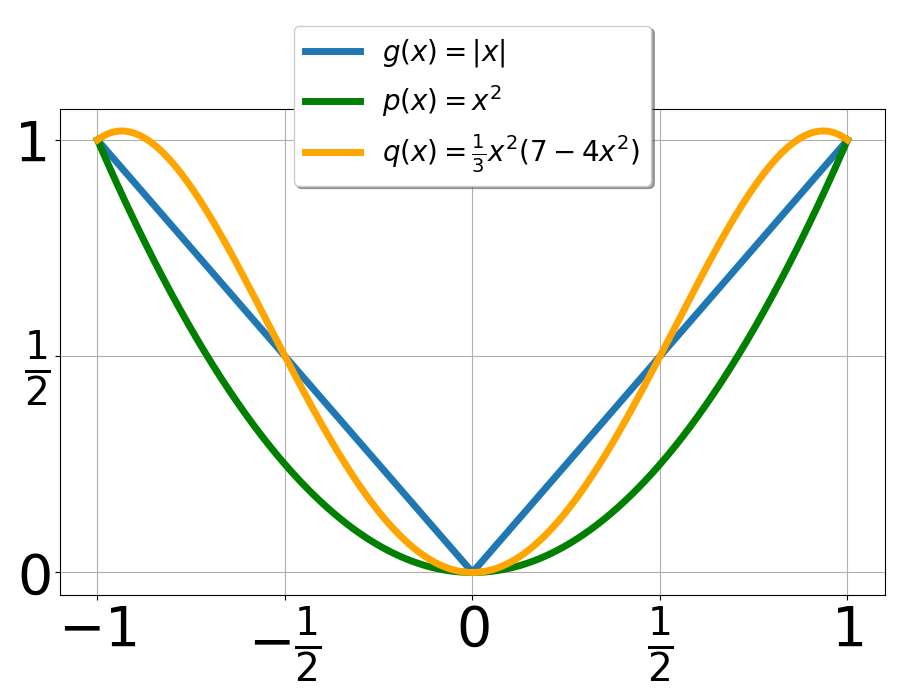
\includegraphics[width=0.8\linewidth]{UA_Section_6_7_Figure_1.png}
        \caption{\( g, p, \) and \( q \) on \( [-1, 1] \)}
        \label{fig:1}
    \end{figure}
    \begin{enumerate}
        \item It is clear that the desired second degree polynomial is \( p(x) = x^2 \). See \Cref{fig:1} for the sketches.

        \item We are looking for a polynomial \( q(x) = a_0 + a_1 x + a_2 x^2 + a_3 x^3 + a_4 x^4 \) such that \( q(-1) = 1, q \paren{ -\tfrac{1}{2} } = \tfrac{1}{2}, q(0) = 0, q \paren{ \tfrac{1}{2} } = \tfrac{1}{2}, \) and \( q(1) = 1 \). The condition \( q(0) = 0 \) immediately gives us \( a_0 = 0 \) and the remaining four conditions give us the linear system
        \[
            \systeme{-a_1 + a_2 - a_3 + a_4 = 1, \tfrac{1}{2} a_1 + \tfrac{1}{4} a_2 - \tfrac{1}{8} a_3 + \tfrac{1}{16} a_4 = \tfrac{1}{2}, \tfrac{1}{2} a_1 + \tfrac{1}{4} a_2 + \tfrac{1}{8} a_3 + \tfrac{1}{16} a_4 = \tfrac{1}{2}, a_1 + a_2 + a_3 + a_4 = 1}.
        \]
        Using Gaussian elimination, or otherwise, this system can be solved to obtain \( a_1 = 0, a_2 = \tfrac{7}{3}, a_3 = 0, \) and \( a_4 = -\tfrac{4}{3} \) and thus \( q(x) = \tfrac{1}{3} x^2 (7 - 4x^2) \). See \Cref{fig:1} for the sketch.
    \end{enumerate}
\end{solution}

\begin{exercise}
\label{ex:4}
    Show that \( f(x) = \sqrt{1 - x} \) has Taylor series coefficients \( a_n \) where \( a_0 = 1 \) and
    \[
        a_n = \frac{-1 \cdot 3 \cdot 5 \cdots (2n - 3)}{2 \cdot 4 \cdot 6 \cdots 2n}
    \]
    for \( n \geq 1 \).
\end{exercise}

\begin{solution}
    We have \( f(0) = a_0 = 1 \) and it is a straightforward calculation to see that
    \[
        f^{(n)}(x) = \frac{-1 \cdot 3 \cdot 5 \cdots (2n - 3)}{2^n} (1 - x)^{-n - 1/2}
    \]
    for \( n \geq 1 \). It follows from this that
    \[
        a_n = \frac{f^{(n)}(0)}{n!} = \frac{-1 \cdot 3 \cdot 5 \cdots (2n - 3)}{2^n n!} = a_n = \frac{-1 \cdot 3 \cdot 5 \cdots (2n - 3)}{2 \cdot 4 \cdot 6 \cdots 2n}
    \]
    for \( n \geq 1 \).
\end{solution}

\begin{exercise}
\label{ex:5}
    \begin{enumerate}
        \item Follow the advice in \href{https://lew98.github.io/Mathematics/UA_Section_6_6_Exercises.pdf}{Exercise 6.6.9} to prove the Cauchy form of the remainder:
        \[
            E_N(x) = \frac{f^{(N + 1)}(c)}{N!} (x - c)^N x
        \]
        for some \( c \) between 0 and \( x \).

        \item Use this result to prove equation (1) is valid for all \( x \in (-1, 1) \).
    \end{enumerate}
\end{exercise}

\begin{solution}
    \begin{enumerate}
        \item See \href{https://lew98.github.io/Mathematics/UA_Section_6_6_Exercises.pdf}{Exercise 6.6.9}.

        \item Suppose \( 0 < \abs{x} < 1 \). For \( n \in \N \), the Cauchy Remainder Theorem implies that there exists some \( c_n \) such that \( 0 < \abs{c_n} < \abs{x} \) and
        \begin{align*}
            E_n(x) &= \frac{f^{(n+1)}(c_n)}{n!} (x - c_n)^n x \\[2mm]
            &= \frac{-1 \cdot 3 \cdots (2n - 3)(2n - 1)}{2^{n+1} n!} (1 - c_n)^{-n - 3/2} (x - c_n)^n x \\[2mm]
            &= -\frac{1}{2} \cdot \frac{1 \cdot 3 \cdots (2n - 3)(2n - 1)}{2 \cdot 4 \cdots (2n - 2)(2n)} \paren{ \frac{x - c_n}{1 - c_n} }^n \frac{x}{(1 - c_n)^{3/2}} \\[2mm]
            &= -\frac{1}{2} \paren{ \prod_{j=1}^n \frac{2j - 1}{2j} } \paren{ \frac{x - c_n}{1 - c_n} }^n \frac{x}{(1 - c_n)^{3/2}}.
        \end{align*}
        Since \( \tfrac{2j - 1}{2j} < 1 \) for each \( 1 \leq j \leq n \), we have \( \prod_{j=1}^n \frac{2j - 1}{2j} < 1 \) and thus
        \[
            \abs{E_n(x)} < \abs{\frac{x - c_n}{1 - c_n}}^n \frac{\abs{x}}{(1 - c_n)^{3/2}};
        \]
        we have used that \( \abs{c_n} < 1 \implies 0 < 1 - c_n < 2 \) to obtain \( \abs{1 - c_n} = 1 - c_n \). Note that
        \[
            c_n \leq \abs{c_n} < \abs{x} \quimplies -\abs{x} < -c_n \quimplies \frac{1}{(1 - c_n)^{3/2}} < \frac{1}{(1 - \abs{x})^{3/2}}.
        \]
        Note further that if \( 0 < c_n < x < 1 \) then
        \[
            x c_n < c_n \quimplies \frac{x - c_n}{1 - c_n} < x \quimplies \abs{\frac{x - c_n}{1 - c_n}} < \abs{x},
        \]
        and if \( -1 < x < c_n < 0 \) then
        \[
            c_n < x c_n \quimplies \frac{c_n - x}{1 - c_n} < -x \quimplies \abs{\frac{x - c_n}{1 - c_n}} < \abs{x}.
        \]
        Combining these inequalities, we see that
        \[
            \abs{E_n(x)} < \frac{\abs{x}^{n+1}}{(1 - \abs{x})^{3/2}}
        \]
        and it follows that \( \lim_{n \to \infty} E_n(x) = 0 \) since \( \abs{x} < 1 \).
    \end{enumerate}
\end{solution}

\begin{exercise}
\label{ex:6}
    \begin{enumerate}
        \item Let
        \[
            c_n = \frac{1 \cdot 3 \cdot 5 \cdots (2n - 1)}{2 \cdot 4 \cdot 6 \cdots 2n}
        \]
        for \( n \geq 1 \). Show \( c_n < \frac{2}{\sqrt{2n + 1}} \).

        \item Use (a) to show that \( \sum_{n=0}^{\infty} a_n \) converges (absolutely, in fact) where \( a_n \) is the sequence of Taylor coefficients generated in \Cref{ex:4}.

        \item Carefully explain how this verifies that equation (1) holds for all \( x \in [-1, 1] \).
    \end{enumerate}
\end{exercise}

\begin{solution}
    \begin{enumerate}
        \item We will prove this by induction. For the base case \( n = 1 \), we have
        \[
            c_1 = \frac{1}{2} < \frac{2}{\sqrt{3}} = \frac{2}{\sqrt{2(1) + 1}}.  
        \]
        Suppose the inequality holds for some \( n \in \N \), so that
        \[
            c_{n+1} = c_n \cdot \frac{2n + 1}{2n + 2} < \frac{2}{\sqrt{2n + 1}} \cdot \frac{2n + 1}{2n + 2} = \frac{2 \sqrt{2n + 1}}{2n + 2}.
        \]
        Now observe that
        \begin{align*}
            \frac{2 \sqrt{2n + 1}}{2n + 2} < \frac{2}{\sqrt{2n + 3}} &\iff \frac{\sqrt{2n + 1}}{2n + 2} < \frac{1}{\sqrt{2n + 3}} \\[2mm]
            &\iff \frac{2n + 1}{4n^2 + 8n + 4} < \frac{1}{2n + 3} \\[2mm]
            &\iff 4n^2 + 8n + 3 < 4n^2 + 8n + 4 \\[2mm]
            &\iff 0 < 1.
        \end{align*}
        Thus \( c_{n+1} < \frac{2}{\sqrt{2n + 3}} \). This completes the induction step and the proof.

        \item Since
        \[
            \sum_{n=0}^{\infty} \abs{a_n} = 1 + \sum_{n=1}^{\infty} \abs{a_n},
        \]
        it will suffice to show that \( \sum_{n=1}^{\infty} \abs{a_n} \) is convergent. Note that for \( n \geq 1 \) we have by part (a)
        \[
            \abs{a_n} = \frac{c_n}{2n - 1} < \frac{2}{(2n - 1) \sqrt{2n + 1}} < \frac{2}{(2n - 1)^{3/2}} \leq \frac{2}{n^{3/2}}.
        \]
        Since the series \( \sum_{n=1}^{\infty} \tfrac{2}{n^{3/2}} \) is convergent (Corollary 2.4.7), we see by comparison that the series \( \sum_{n=1}^{\infty} \abs{a_n} \) is convergent.

        \item Part (b) shows that the power series \( \sum_{n=0}^{\infty} a_n x^n \) converges absolutely at the points \( x = -1 \) and \( x = 1 \). It follows from Abel's Theorem (Theorem 6.5.4) that the power series converges uniformly and hence is continuous on \( [-1, 1] \). Thus the function \( h : [-1, 1] \to \R \) given by
        \[
            h(x) = \sqrt{1 - x} - \sum_{n=0}^{\infty} a_n x^n
        \]
        is continuous on its domain and, by \Cref{ex:5}, satisfies \( h(x) = 0 \) for all \( x \in (-1, 1) \). It must then be the case that \( h(-1) = h(1) = 0 \) also.
    \end{enumerate}
\end{solution}

\begin{exercise}
\label{ex:7}
    \begin{enumerate}
        \item Use the fact that \( \abs{a} = \sqrt{a^2} \) to prove that, given \( \epsilon > 0 \), there exists a polynomial \( q(x) \) satisfying
        \[
            \abs{\abs{x} - q(x)} < \epsilon
        \]
        for all \( x \in [-1, 1] \).

        \item Generalize this conclusion to an arbitrary interval \( [a, b] \).
    \end{enumerate}
\end{exercise}

\begin{solution}
    \begin{enumerate}
        \item Note that \( x \in [-1, 1] \) implies that \( 1 - x^2 \in [0, 1] \) and thus by \Cref{ex:6} we have
        \[
            \sqrt{1 - (1 - x^2)} = \sum_{n=0}^{\infty} a_n (1 - x^2)^n.
        \]
        As we showed in \Cref{ex:6} this convergence is uniform, so there exists an \( N \in \N \) such that
        \[
            \abs{\sqrt{1 - (1 - x^2)} - \sum_{n=0}^{N} a_n (1 - x^2)^n} = \abs{\abs{x} - \sum_{n=0}^{N} a_n (1 - x^2)^n} < \epsilon
        \]
        for all \( x \in [-1, 1] \). Thus the desired polynomial is \( q(x) = \sum_{n=0}^{N} a_n (1 - x^2)^n \).

        \item For \( a < b \) and \( \epsilon > 0 \), we would like to find a polynomial \( p \) such that \( \abs{\abs{x} - p(x)} < \epsilon \) for all \( x \in [a, b] \). Let \( c = \max \{ \abs{a}, \abs{b} \} \) and note that \( c > 0 \). Note further that \( x \in [a, b] \) implies that \( \tfrac{x}{c} \in [-1, 1] \) and thus by part (a) there exists a polynomial \( q \) such that
        \[
            \abs{ \abs{ \frac{x}{c} } - q \paren{ \frac{x}{c} } } < \frac{\epsilon}{c} \tag{1}
        \]
        for all \( \tfrac{x}{c} \in [-1, 1] \), i.e\ for all \( x \in [-c, c] \). Let \( p \) be the polynomial given by \( p(x) = c q \paren{ \tfrac{x}{c} } \). It follows from (1) that
        \[
            \abs{ \abs{x} - p(x) } < \epsilon
        \]
        for all \( x \in [-c, c] \) and hence in particular for all \( x \in [a, b] \).
    \end{enumerate}
\end{solution}

\begin{exercise}
\label{ex:8}
    \begin{enumerate}
        \item Fix \( a \in [-1, 1] \) and sketch
        \[
            h_a(x) = \frac{1}{2} ( \abs{x - a} + (x - a) )
        \]
        over \( [-1, 1] \). Note that \( h_a \) is polygonal and satisfies \( h_a(x) = 0 \) for all \( x \in [-1, a] \).

        \item Explain why we know \( h_a(x) \) can be uniformly approximated with a polynomial on \( [-1, 1] \).

        \item Let \( \phi \) be a polygonal function that is linear on each subinterval of the partition
        \[
            -1 = a_0 < a_1 < a_2 < \cdots < a_n = 1.
        \]
        Show there exist constants \( b_0, b_1, \ldots, b_{n-1} \) so that
        \[
            \phi(x) = \phi(-1) + b_0 h_{a_0}(x) + b_1 h_{a_1}(x) + \cdots + b_{n-1} h_{a_{n-1}}(x)
        \]
        for all \( x \in [-1, 1] \).

        \item Complete the proof of WAT for the interval \( [-1, 1] \), and then generalize to an arbitrary interval \( [a, b] \).
    \end{enumerate}
\end{exercise}

\begin{solution}
    \begin{figure}[H]
        \centering
        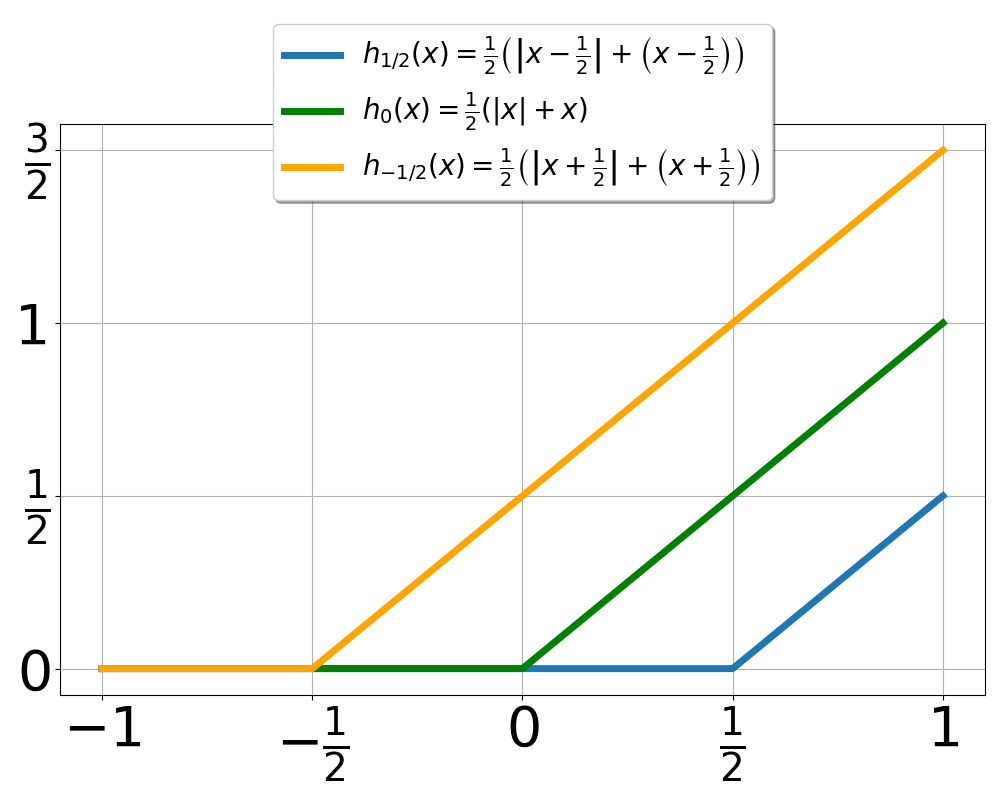
\includegraphics[width=0.8\linewidth]{UA_Section_6_7_Figure_2.png}
        \caption{\( h_{1/2}, h_0, \) and \( h_{1/2} \) on \( [-1, 1] \)}
        \label{fig:2}
    \end{figure}
    \begin{enumerate}
        \item See \Cref{fig:2} for a sketch of \( h_{1/2}, h_0, \) and \( h_{1/2} \) on \( [-1, 1] \).

        \item From \Cref{ex:7} (b), for a given \( \epsilon > 0 \) we know that there exists a polynomial \( q \) such that
        \[
            \abs{\abs{x - a} - q(x - a)} < 2 \epsilon 
        \]
        for all \( x \in [-1, 1] \). Let \( p(x) = \tfrac{1}{2} q(x - a) + \tfrac{1}{2} (x - a) \) and observe that
        \[
            \abs{h_a(x) - p(x)} = \frac{1}{2} \abs{ \abs{x - a} - q(x - a) } < \epsilon
        \]
        for all \( x \in [-1, 1] \).

        \item For \( 0 \leq j \leq n - 1 \), the polygonal function \( \phi \) is given by a line segment on the subinterval \( [a_j, a_{j+1}] \); let \( m_j \) be the slope of this line segment, i.e.\
        \[
            m_j = \frac{\phi(a_{j+1}) - \phi(a_j)}{a_{j+1} - a_j}.  
        \]
        Now set \( b_0 = m_0 \) and \( b_j = m_j - m_{j-1} \) for \( 1 \leq j \leq n - 1 \) and let \( \psi : [-1, 1] \to \R \) be given by
        \[
            \psi(x) = \phi(a_0) + b_0 h_{a_0}(x) + b_1 h_{a_1}(x) + \cdots + b_{n-1} h_{a_{n-1}}(x).
        \]
        Our aim is to show that \( \phi(x) = \psi(x) \) for all \( x \in [-1, 1] \). For such an \( x \), we have \( x \in [a_j, a_{j+1}] \) for some \( 0 \leq j \leq n - 1 \). Note that
        \[
            \phi(x) = \phi(a_j) + m_j (x - a_j).
        \]
        Note further that \( h_{a_0}(x) = x - a_0, \ldots, h_{a_j}(x) = x - a_j \) and that \( h_{a_{j+1}}(x) = \cdots = h_{a_{n-1}}(x) = 0 \). Thus
        \begin{align*}
            \psi(x) &= \phi(a_0) + b_0 h_{a_0}(x) + b_1 h_{a_1}(x) + \cdots + b_j h_{a_j}(x) \\[2mm]
            &= \phi(a_0) + m_0 (x - a_0) + (m_1 - m_0)(x - a_1) + \cdots + (m_j - m_{j-1}) (x - a_j) \\[2mm]
            &= \phi(a_0) + m_0 (a_1 - a_0) + m_1 (a_2 - a_1) + \cdots + m_{j-1} (a_j - a_{j-1}) + m_j (x - a_j) \\[2mm]
            &= \phi(a_1) + m_1 (a_2 - a_1) + \cdots + m_{j-1} (a_j - a_{j-1}) + m_j (x - a_j) \\[2mm]
            &= \cdots \\[2mm]
            &= \phi(a_j) + m_j (x - a_j) \\[2mm]
            &= \phi(x).
        \end{align*}

        \item Let \( f : [-1, 1] \to \R \) be continuous and let \( \epsilon > 0 \) be given. By Theorem 6.7.3 (see \Cref{ex:2}), there exists a polygonal function \( \phi : [-1, 1] \to \R \) which is linear on each subinterval of some partition
        \[
            -1 = a_0 < a_1 < \cdots < a_n = 1
        \]
        and which satisfies \( \abs{f(x) - \phi(x)} < \tfrac{\epsilon}{2} \) for all \( x \in [-1, 1] \). By part (c), there exist constants \( b_0, \ldots, b_{n-1} \) such that
        \[
            \phi(x) = \phi(a_0) + b_0 h_{a_0}(x) + \cdots + b_{n-1} h_{a_{n-1}}(x)
        \]
        for all \( x \in [-1, 1] \). Furthermore, by part (b), for each \( 0 \leq j \leq n - 1 \) there exists a polynomial \( p_j \) such that
        \[
            \abs{h_{a_j}(x) - p_j(x)} < \frac{\epsilon}{2n(1 + \abs{b_j})}.
        \]
        Let \( p \) be the polynomial given by
        \[
            p(x) = \phi(a_0) + b_0 p_0(x) + \cdots + b_{n-1} p_{n-1}(x)
        \]
        and observe that for any \( x \in [-1, 1] \) we have
        \begin{align*}
            \abs{\phi(x) - p(x)} &= \abs{b_0 h_{a_0}(x) + \cdots + b_{n-1} h_{a_{n-1}}(x) - b_0 p_0(x) - \cdots - b_{n-1} p_{n-1}(x)} \\[2mm]
            &\leq \abs{b_0} \abs{h_{a_0}(x) - p_0(x)} + \cdots + \abs{b_{n-1}} \abs{h_{a_{n-1}}(x) - p_{n-1}(x)} \\[2mm]
            &< \frac{\epsilon \abs{b_0}}{2n(1 + \abs{b_0})} + \cdots + \frac{\epsilon \abs{b_{n-1}}}{2n(1 + \abs{b_{n-1}})} \\[2mm]
            &< \frac{\epsilon}{2n} + \cdots + \frac{\epsilon}{2n} \\[2mm]
            &= \frac{\epsilon}{2}.
        \end{align*}
        It now follows that for any \( x \in [-1, 1] \) we have
        \[
            \abs{f(x) - p(x)} \leq \abs{f(x) - \phi(x)} + \abs{\phi(x) - p(x)} < \frac{\epsilon}{2} + \frac{\epsilon}{2} = \epsilon.
        \]

        We can now prove the general case. For \( a < b \), let \( f : [a, b] \to \R \) be continuous and let \( \epsilon > 0 \) be given. We would like to find a polynomial \( p \) such that \( \abs{f(x) - p(x)} < \epsilon \) for all \( x \in [a, b] \). Note that the function
        \[
            \begin{array}{>{\displaystyle}r >{\displaystyle}c >{\displaystyle}l}
                [-1, 1] & \to & [a, b] \\[2mm]
                x & \mapsto & \frac{b - a}{2}(x + 1) + a
            \end{array}
        \]
        is a continuous bijection with inverse
        \[
            \begin{array}{>{\displaystyle}r >{\displaystyle}c >{\displaystyle}l}
                [a, b] & \to & [-1, 1] \\[2mm]
                x & \mapsto & \frac{2(x - a)}{b - a} - 1.
            \end{array}
        \]
        Thus \( g : [-1, 1] \to \R \) given by
        \[
            g(x) = f \paren{ \frac{b - a}{2} (x + 1) + a }  
        \]
        is well-defined and, as a composition of continuous functions, is continuous on \( [-1, 1] \). It follows from our previous discussion that there exists a polynomial \( q \) such that \( \abs{g(x) - q(x)} < \epsilon \) for all \( x \in [-1, 1] \). Let \( p \) be the polynomial defined by
        \[
            p(x) = q \paren{ \frac{2(x - a)}{b - a} - 1 }.
        \]
        Since \( x \in [a, b] \) implies that \( \tfrac{2(x - a)}{b - a} - 1 \in [-1, 1] \), we have
        \[
            \abs{ g \paren{ \frac{2(x - a)}{b - a} - 1 } - q \paren{ \frac{2(x - a)}{b - a} - 1 }} = \abs{f(x) - p(x)} < \epsilon
        \]
        for all \( x \in [a, b] \).
    \end{enumerate}
\end{solution}

\begin{exercise}
\label{ex:9}
    \begin{enumerate}
        \item Find a counterexample which shows that WAT is not true if we replace the closed interval \( [a, b] \) with the open interval \( (a, b) \).

        \item What happens if we replace \( [a, b] \) with the closed set \( [a, \infty) \). Does the theorem still hold?
    \end{enumerate}
\end{exercise}

\begin{solution}
    \begin{enumerate}
        \item Consider \( f : (0, 1) \to \R \) given by \( f(x) = x^{-1} \). Since any polynomial is bounded on \( (0, 1) \), if we could uniformly approximate \( f \) with a polynomial on \( (0, 1) \) then we would have that \( f \) is bounded on \( (0, 1) \), which is not true.

        \item The theorem does not hold. Consider \( g : [0, \infty) \to \R \) given by \( g(x) = \sin(x) \). Evidently \( g \) cannot be uniformly approximated by a constant polynomial on \( [0, \infty) \), and for a non-constant polynomial \( p \) we have \( \lim_{x \to \infty} \abs{p(x)} = +\infty \), whereas \( \abs{g(x)} \leq 1 \) for all \( x \in [0, \infty) \); it follows that we cannot uniformly approximate \( g \) with a non-constant polynomial on \( [0, \infty) \) either.
    \end{enumerate}
\end{solution}

\begin{exercise}
\label{ex:10}
    Is there a countable subset of polynomials \( \mathcal{C} \) with the property that every continuous function on \( [a, b] \) can be uniformly approximated by polynomials from \( \mathcal{C} \)?
\end{exercise}

\begin{solution}
    There is such a countable subset. Let \( \poly(\R) \) be the collection of polynomials with real coefficients, let \( \poly(\Q) \subseteq \poly(\R) \) be the collection of polynomials with rational coefficients, and for each \( n \geq 0 \) let \( \poly_n(\Q) \subseteq \poly(\Q) \) be the collection of polynomials of degree \( n \) with rational coefficients. Then \( \poly_0(\Q) \) is in bijection with \( \Q \setminus \{ 0 \} \) and \( \poly_n(\Q) \) is in bijection with \( \Q^{n-1} \times \paren{ \Q \setminus \{ 0 \} } \) for each \( n \geq 1 \). Thus each \( \poly_n(\Q) \) is countable and it follows from the expression
    \[
        \poly(\Q) = \{ 0 \} \cup \bigcup_{n=0}^{\infty} \poly_n(\Q)
    \]
    (by 0 we mean the zero polynomial) and Theorem 1.5.8 (ii) that \( \poly(\Q) \) is countable.

    Now let \( a < b \) be given and set \( M = \max \{ \abs{a}, \abs{b}, 1 \} \). Suppose \( f : [a, b] \to \R \) is continuous and let \( \epsilon > 0 \) be given. By the Weierstrass Approximation Theorem, there exists a polynomial
    \[
        p(x) = a_n x^n + a_{n-1} x^{n-1} + \cdots + a_1 x + a_0 \in \poly(\R)
    \]
    such that \( \abs{f(x) - p(x)} < \tfrac{\epsilon}{2} \) for all \( x \in [a, b] \). By the density of \( \Q \) in \( \R \), we can choose rational numbers \( b_n, b_{n-1}, \ldots, b_1, b_0 \) such that \( \abs{a_j - b_j} < \tfrac{\epsilon}{2M^n(n+1)} \) for each \( 0 \leq j \leq n \). Set
    \[
        q(x) = b_n x^n + b_{n-1} x^{n-1} + \cdots + b_1 x + b_0 \in \poly(\Q)
    \]
    and observe that for any \( x \in [a, b] \) we have
    \begin{align*}
        \abs{p(x) - q(x)} &= \abs{(a_n - b_n) x^n + (a_{n-1} - b_{n-1}) x^{n-1} + \cdots + (a_1 - b_1) x + (a_0 - b_0)} \\[2mm]
        &\leq \abs{a_n - b_n} \abs{x}^n + \abs{a_{n-1} - b_{n-1}} \abs{x}^{n-1} + \cdots + \abs{a_1 - b_1} \abs{x} + \abs{a_0 - b_0} \\[2mm]
        &\leq \abs{a_n - b_n} M^n + \abs{a_{n-1} - b_{n-1}} M^{n-1} + \cdots + \abs{a_1 - b_1} M + \abs{a_0 - b_0} \\[2mm]
        &\leq \abs{a_n - b_n} M^n + \abs{a_{n-1} - b_{n-1}} M^n + \cdots + \abs{a_1 - b_1} M^n + \abs{a_0 - b_0} M^n \\[2mm]
        &< \frac{\epsilon}{2(n+1)} + \frac{\epsilon}{2(n+1)} + \cdots + \frac{\epsilon}{2(n+1)} + \frac{\epsilon}{2(n+1)} \\[2mm]
        &= \frac{\epsilon}{2}.
    \end{align*}
    It follows that
    \[
        \abs{f(x) - q(x)} \leq \abs{f(x) - p(x)} + \abs{p(x) - q(x)} < \frac{\epsilon}{2} + \frac{\epsilon}{2} = \epsilon
    \]
    for any \( x \in [a, b] \). Thus the desired countable subset \( \mathcal{C} \) is \( \poly(\Q) \).
\end{solution}

\begin{exercise}
\label{ex:11}
    Assume that \( f \) has a continuous derivative on \( [a, b] \). Show that there exists a polynomial \( p(x) \) such that
    \[
        \abs{f(x) - p(x)} < \epsilon \quand \abs{f'(x) - p'(x)} < \epsilon
    \]
    for all \( x \in [a, b] \).
\end{exercise}

\begin{solution}
    By assumption \( f' \) is continuous on \( [a, b] \), so the Weierstrass Approximation Theorem yields a polynomial \( q \) such that \( \abs{f'(x) - q(x)} < \tfrac{\epsilon}{b - a} \) for all \( x \in [a, b] \). Let \( p \) be the polynomial which satisfies \( p' = q \) and \( p(a) = f(a) \) and let \( g : [a, b] \to \R \) be given by \( g(x) = f(x) - p(x) \). Then \( g(a) = 0 \) and \( g'(x) = f'(x) - q(x) \), so that \( \abs{g'(x)} < \tfrac{\epsilon}{b - a} \) for all \( x \in [a, b] \). Let \( x \in (a, b] \) be given. By the Mean Value Theorem (Theorem 5.3.2), there exists some \( c \in (a, x) \) such that
    \[
        \abs{f(x) - p(x)} = \abs{g(x) - g(a)} = \abs{g'(c) (x - a)} \leq (b - a) \frac{\epsilon}{b - a} = \epsilon.
    \]
\end{solution}

\noindent \hrulefill

\noindent \hypertarget{ua}{\textcolor{blue}{[UA]} Abbott, S. (2015) \textit{Understanding Analysis.} 2\ts{nd} edition.}

\end{document}